%Este trabalho está licenciado sob a Licença Creative Commons Atribuição-CompartilhaIgual 3.0 Não Adaptada. Para ver uma cópia desta licença, visite http://creativecommons.org/licenses/by-sa/3.0/ ou envie uma carta para Creative Commons, PO Box 1866, Mountain View, CA 94042, USA.

%\documentclass[main.tex]{subfiles}
%\begin{document}

\chapter{Derivação Numérica}\index{derivação}

Nesta seção, discutiremos sobre estratégias numéricas para o cálculo aproximação de derivadas de funções reais. Com as técnicas que abordaremos é possível o cálculo aproximado da derivada de uma função, mesmo quando conhecemos apenas um conjunto de pontos discretos $\{x_i, y_i\}_{i=1}^n$ e não conhecemos a lei de correspondência $y = f(x)$ da função em questão.

Começamos discutindo sobre as chamadas \emph{aproximações por diferenças finitas}\index{aproximações por diferenças finitas} e, então, discutimos sobre aproximações de derivadas via ajuste ou interpolação.

\section{Diferenças finitas}\index{diferenças finitas}

A técnica de \emph{diferenças finitas}\index{diferenças finitas} consiste em aproximar a derivada de uma função via fórmulas discretas que requerem apenas um conjunto finito de pares ordenados $\left\{\left(x_i, y_i=f(x_i)\right)\right\}_{i=1}^n$. As chamadas fórmulas de diferenças finitas podem ser obtidas de várias formas. Começamos discutindo a mais básica delas, a chamada fórmula de diferenças progressiva de ordem 1.

Seja dada uma função diferenciável $y = f(x)$. A derivada $f'(x_0)$ da função $f(x)$ no ponto $x_0$ é dada por
\begin{equation*}
  f'(x_0)=\lim_{h\to 0}\frac{f(x_0+h)-f(x_0)}{h}.
\end{equation*}
Deste limite, tomando $h\neq 0$ pequeno (não muito pequeno para evitar o cancelamento catastrófico), é esperado que possamos obter uma aproximação razoável para $f'(x_0)$ calculando:
\begin{equation}\label{eq:dp}
  D_{+,h}f(x_0) := \frac{f(x_0+h)-f(x_0)}{h} \approx f'(x_0).
\end{equation}
Aqui, $D_{+,h}f(x_0)$ é a chamada fórmula de diferenças progressiva de ordem 1 (ou de primeira ordem).

\begin{ex}\label{ex:dp}
Use a fórmula de diferenças finitas progressiva de ordem 1, calcule aproximações da derivada de $f(x)=\cos(x)$ no ponto $x=1$ usando $h=10^{-1}$, $10^{-2}$, $10^{-3}$, $10^{-4}$, $10^{-12}$ e $10^{-14}$. Então, compute o erro $|D_{+,h}f(1)-f'(1)|$ obtido com cada valor de $h$.
\end{ex}
\begin{sol}
Usando a fórmula de diferenças dada na equação~\eqref{eq:dp}, devemos calcular:
\begin{equation*}
  D_{+,h}f(1) = \frac{\cos(1 + h) - \cos(1)}{h}
\end{equation*}
para cada valor de $h$ solicitado. Fazendo isso, obtemos:
\begin{equation*}
  \begin{array}{r|c|c}
    h & Df(1) & |f'(1) - D_{+,h}F(1)| \\ \hline
    10^{-1} & -8,67062(-01) & 2,55909(-02)\\
    10^{-2} & -8,44158(-01) & 2,68746(-03)\\
    10^{-3} & -8,41741(-01) & 2,70011(-04)\\
    10^{-4} & -8,41498(-01) & 2,70137(-05) \\
    10^{-12} & -8,41549(-01) & 7,80679(-05)\\
    10^{-14} & -8,43769(-01) & 2,29851(-03) \\\hline
    \multicolumn{3}{c}{}
  \end{array}
\end{equation*}

\ifisscilab
No \verb+Scilab+, podemos calcular a aproximação da derivada $f'(1)$ com $h=0,1$ usando as seguintes linhas de código:
\begin{verbatim}
--> deff('y = f(x)','y = cos(x)')
--> x0 = 1
--> h = 0.1
--> df = (f(x0+h) - f(x0))/h
\end{verbatim}
E, similarmente, para outros valores de $x_0$ e $h$.
\fi
\end{sol}

\begin{figure}
  \centering
  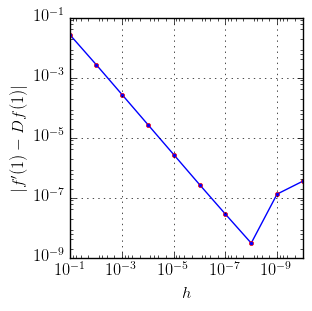
\includegraphics{./cap_derivacao/pics/ex_derivacao/ex_derivacao}
  \caption{Erro da aproximação da derivada numérica no Exemplo~\ref{ex:dp}.}
  \label{fig:ex_derivacao}
\end{figure}

Exploremos o Exemplo~\ref{ex:dp} um pouco mais. Observamos que, para valores moderados de $h$, o erro $|f'(1)-D_{+,h}f(1)|$ diminui linearmente com $h$ (veja Figura~\ref{fig:ex_derivacao}). Isto é consequência da ordem de truncamento da fórmula de diferenças finitas aplicada (que é de ordem 1). Porém, para valores muito pequenos de $h < 10^{-8}$, o erro passa a aumentar quando diminuímos $h$. Isto é devido ao efeito de cancelamento catastrófico.

\subsection{Obtenção de fórmulas de diferenças via série de Taylor}

Podemos construir fórmulas de diferenças finitas para uma função $f(x)$ (suave) no ponto $x = x_0$ a partir de sua expansão em série de Taylor. Em alguns casos, este procedimento acaba por nos fornecer, também, a ordem de truncamento da fórmula.

\subsubsection{Fórmula de diferenças finitas progressiva de ordem 1}\index{diferenças finitas!progressiva}

A fórmula de diferenças finitas progressiva pode ser obtida fazendo a seguinte expansão em série de Taylor:
\begin{equation*}
  f(x_0+h) = f(x_0) + hf'(x_0) + h^2\frac{f''(\xi)}{2},\quad h>0, \xi\in(x_0,x_0+h).
\end{equation*}
Então, isolando $f'(x_0)$, obtemos:
\begin{equation*}
  f'(x_0) = \underbrace{\frac{f(x_0+h) - f(x_0)}{h}}_{D_{+,h}} - \underbrace{h\frac{f''(\xi)}{2}}_{\text{truncamento}},
\end{equation*}
o que corrobora que o erro de truncamento da fórmula de diferença finitas progressiva:
\begin{equation*}
  D_{+,h}f(x_0) := \frac{f(x_0+h)-f(x_0)}{h}  
\end{equation*}
é de ordem $h$

\subsubsection{Fórmula de diferenças finitas regressiva de ordem 1}\index{diferenças finitas!regressiva}

A fórmula de diferenças finitas regressiva também pode ser obtida fazendo, agora, a seguinte expansão em série de Taylor:
\begin{equation*}
  f(x_0-h) = f(x_0) - hf'(x_0) + h^2\frac{f''(\xi)}{2},\quad h>0, \xi\in(x_0, x_0+h).
\end{equation*}
Então, isolando $f'(x_0)$, obtemos:
\begin{equation*}
  f'(x_0) = \underbrace{\frac{f(x_0) - f(x_0-h)}{h}}_{D_{-,h}} + h\frac{f''(\xi)}{2}.
\end{equation*}
Desta equação, temos que a fórmula:
\begin{equation*}
  D_{-,h}f(x_0) := \frac{f(x_0)-f(x_0-h)}{h},
\end{equation*}
a qual é chamada de fórmula de diferenças finitas regressiva tem erro de truncamento da ordem $h$.

\subsubsection{Fórmula de diferenças finitas central de ordem 2}\index{diferenças finitas!central}

A fórmula de diferenças finitas central pode-se obter de duas expansões em série de Taylor: uma progressiva e outra regressiva. Seguem as expansões:
\begin{equation*}
  \begin{split}
    f(x_0+h) &= f(x_0) + hf'(x_0) + h^2f''(x_0) + h^3\frac{f'''(\xi_{+})}{3!},\\
    f(x_0-h) &= f(x_0) - hf'(x_0) + h^2f''(x_0) + h^3\frac{f'''(\xi_{-})}{3!}
  \end{split}
\end{equation*}
Fazendo a primeira equação menos a segunda, obtemos:
\begin{equation*}
  f(x_0+h)-f(x_0-h) = 2hf'(x_0) + h^{3}\left(\frac{f'''(\xi_{+}) - f'''(\xi_{-})}{3!}\right).
\end{equation*}
Então, isolando $f'(x_0)$ obtemos:
\begin{equation*}
  f'(x_0) = \underbrace{\frac{f(x_0+h) - f(x_0-h)}{2h}}_{D_{0,h}} - h^2\left(\frac{f'''(\xi_+) - f'''(\xi_-)}{3!}\right).
\end{equation*}
Desta equação, temos que a fórmula:
\begin{equation*}
  D_{0,h}f(x_0) := \frac{f(x_0+h)-f(x_0-h)}{2h},
\end{equation*}
a qual é chamada de \emph{fórmula de diferenças finitas central}\index{diferenças finitas!central} e tem erro de truncamento da ordem $2$.

\begin{ex}
Calcule a derivada numérica da função $f(x)=\cos(x)$ no ponto $x=1$ usando diferenças progressivas, diferenças regressivas e diferenças centrais com $h=0,1$, $h=0,01$ e $h=0,001$.
\end{ex}
\begin{sol}
A tabela abaixo mostra a derivada numérica para cada valor de $h$.
\begin{center}
\begin{tabular}{|l|c|} \hline
  Diferenças & h=0,1 \\ \hline
  Progressivas & $\displaystyle -0,8670618$ \\
  Regressivas  & $\displaystyle \frac{\cos(1)-\cos(0,9)}{0,1} = -0,8130766$ \\
  Centrais     & $\displaystyle \frac{\cos(1,1)-\cos(0,9)}{0,2} = -0,8400692$ \\ \hline
  Diferenças & h=0,01 \\ \hline
  Progressivas & $\displaystyle -0,8441584$ \\
  Regressivas  & $\displaystyle \frac{\cos(1)-\cos(0,99)}{0,01} = -0,8387555$ \\
  Centrais     & $\displaystyle \frac{\cos(1,01)-\cos(0,99)}{0,02} = -0,8414570$ \\ \hline
  Diferenças & h=0,01 \\ \hline
  Progressivas & $\displaystyle -0,841741$ \\
  Regressivas  & $\displaystyle \frac{\cos(1)-\cos(0,999)}{0,001} = -0,8412007$ \\
  Centrais     & $\displaystyle \frac{\cos(1,001)-\cos(0,999)}{0,002} = -0,8414708$ \\ \hline
\end{tabular}  
\end{center}  
\end{sol}

% \subsection{Erros de truncamento}\index{erros!truncamento}
% Seja $D_{+,h}f(x_0)$ a aproximação da derivada de $f$ em $x_0$ por diferenças progressivas, $D_{-,h}f(x_0)$ a aproximação por diferenças regressivas e $D_{0,h}f(x_0)$ a aproximação por diferenças centrais, então
% \begin{eqnarray*}
% D_{+,h}f(x_0)-f'(x_0)&=&\frac{f(x_0+h)-f(x_0)}{h}-f'(x_0)\\
% &=&\frac{f(x_0)+hf'(x_0)+\frac{h^2}{2}f''(x_0)+O(h^3)-f(x_0)}{h}-f'(x_0)\\
% &=&\frac{h}{2}f''(x_0)+O(h^2)=O(h).\\
% \end{eqnarray*}
% Analogamente:
% \begin{eqnarray*}
% D_{-,h}f(x_0)-f'(x_0)&=&\frac{f(x_0)-f(x_0-h)}{h}-f'(x_0)\\
% &=&\frac{f(x_0)-\left(f(x_0)-hf'(x_0)+\frac{h^2}{2}f''(x_0)+O(h^3)\right)}{h}-f'(x_0)\\
% &=&-\frac{h}{2}f''(x_0)+O(h^2)=O(h).\\
% \end{eqnarray*}
% Também:
% \begin{eqnarray*}
% D_{0,h}f(x_0)-f'(x_0)&=& \frac{f(x_0+h)-f(x_0-h)}{2h}-f'(x_0)\\
% &=& \frac{f(x_0)+hf'(x_0)+\frac{h^2}{2}f''(x_0)+O(h^3)}{2h} \\
% &-& \frac{f(x_0)-hf'(x_0)+\frac{h^2}{2}f''(x_0)+O(h^3)}{2h}-f'(x_0)\\
% &=& O(h^2).
% \end{eqnarray*}

\begin{ex}
Calcule a derivada numérica e o erro de truncamento de $f(x)=e^{-x}$ em $x=1,5$ pela fórmula de diferença progressiva para $h=0,1$, $h=0,01$ e $h=0,001$.
\end{ex}
\begin{sol}
Como $|f''(x)|=|e^{-x}|<1$, então $|f'_+(x_0)-f'(x_0)|<\frac{h}{2}$.
$$
\begin{array}{|c|c|c|}\hline
 h&\hbox{diferenças progressivas} & \hbox{erro}=\frac{h}{2}\\\hline
0,1&- 0,2123364 & 0,05\\\hline
0,01 &- 0,2220182 & 0,005\\\hline
0,001 &- 0,2230186 & 0,0005\\\hline
\multicolumn{3}{c}{}
\end{array}
$$
O valor exato da derivada é $f'(1,5)=-0,2231302$.
\end{sol}

\subsection{Erros de arredondamento}\index{erros!arredondamento}
Para entender como os erros de arredondamento se propagam ao calcular as derivadas numéricas vamos considerar o operador de diferenças finitas progressivas
$$
D_{+,h}f(x) =\frac{f(x+h)-f(x)}{h}.
$$
Nesse contexto temos o valor exato $f'(x)$ para a derivada, a sua aproximação numérica $D_{+,h}f(x)$ e a representação em número de máquina do operador $D_{+,h}f(x)$ que denotaremos por $\overline{D_{+,h}f(x)}$. Seja $\varepsilon(x,h)$ o erro de arredondamento ao calcularmos a derivada e consideremos
$$
\overline{D_{+,h}f(x)}=D_{+,h}f(x)(1+\varepsilon(x,h))=\frac{\overline{f(x+h)}-\overline{f(x)}}{h}(1+\varepsilon(x,h)).
$$
Também, consideremos
$$
|\overline{f(x+h)}-f(x+h)|=\delta(x,h)\leq \delta
$$
e
$$
|\overline{f(x)}-f(x)|=\delta(x,0)\leq \delta,
$$
onde $\overline{f(x+h)}$ e $\overline{f(x)}$ são as representação em ponto flutuante dos números $f(x+h)$ e $f(x)$, respectivamente. A diferença do valor da derivada e sua aproximação representada em ponto flutuante pode ser estimada da seguinte forma:
\begin{eqnarray*}
\left|f'(x)-\overline{D_{+,h}f(x)}\right|&=& \left| f'(x)-\frac{\overline{f(x+h)}-\overline{f(x)}}{h}(1+\varepsilon(x,h)) \right|\\
&=& \left| f'(x)-\left(\frac{\overline{f(x+h)}-\overline{f(x)}}{h}+\frac{f(x+h)-f(x+h)}{h}\right.\right. \\
&+& \left.\left.\frac{f(x)-f(x)}{h}\right)(1+\varepsilon) \right|\\
&=& \left| f'(x)+\left(-\frac{f(x+h)-f(x)}{h}-\frac{\overline{f(x+h)}-f(x+h)}{h}\right.\right.\\
&+& \left.\left. \frac{\overline{f(x)}-f(x)}{h}\right)(1+\varepsilon) \right|\\
&\leq& \left|f'(x)-\frac{f(x+h)-f(x)}{h}\right| +\left(\left|\frac{\overline{f(x+h)}-f(x+h)}{h}\right|\right.\\
&+&\left.\left|\frac{\overline{f(x)}-f(x)}{h}\right| \right)|1+\varepsilon| + \left|\frac{f(x+h)-f(x)}{h}\right|\varepsilon\\
&\leq& Mh +\left(\left|\frac{\delta}{h}\right|+\left|\frac{\delta}{h}\right| \right)|1+\varepsilon| +|f'(x)|\varepsilon\\
&\leq& Mh +\left(\frac{2\delta}{h}\right)|1+\varepsilon| +|f'(x)|\varepsilon
\end{eqnarray*}
onde
$$
M=\frac{1}{2}\max_{x\leq y\leq x+h}|f''(y)|
$$
está relacionado com o erro de truncamento.

Esta estimativa mostra que se o valor de $h$ for muito pequeno o erro ao calcular a aproximação numérica cresce. Isso nos motiva a procurar o valor ótimo de $h$ que minimiza o erro.

\begin{ex}Estude o comportamento da derivada de $f(x)=e^{-x^2}$ no ponto $x=1,5$ quando $h$ fica pequeno.
\end{ex}
\begin{sol}
Segue a tabela com os valores da derivada para vários valores de $h$.
\begin{tiny}
\begin{equation*}
\begin{array}{|c|c|c|c|c|c|c|}
\hline
h&10^{-2}&10^{-4}&10^{-6}&10^{-7}&10^{-8}&10^{-9}\\
\hline
D_{+,h}f(1,5)& - 0,3125246&- 0,3161608 &- 0,3161973&- 0,3161976&- 0,3161977&- 0,3161977 \\
\hline
\end{array}  
\end{equation*}  
\begin{equation*}
\begin{array}{|c|c|c|c|c|c|c|}
\hline
h&10^{-10}&10^{-11}&10^{-12}&10^{-13}&10^{-14}&10^{-15}\\
\hline
D_{+,h}f(1,5)&- 0,3161976&- 0,3161971&- 0,3162332&- 0,3158585&- 0,3178013&- 0,3747003\\
\hline
\end{array}
\end{equation*}
\begin{equation*}
\begin{array}{|c|c|c|c|c|c|c|}
\hline
h&10^{-2}&10^{-4}&10^{-6}&10^{-7}&10^{-8}&10^{-9}\\
\hline
D_{+,h}f(1,5)& - 0,3125246&- 0,3161608 &- 0,3161973&- 0,3161976&- 0,3161977&- 0,3161977 \\
\hline
\end{array}  
\end{equation*}
\end{tiny}

Observe que o valor exato é $-0,3161977$ e o $h$ ótimo é algo entre $10^{-8}$ e $10^{-9}$.  
\end{sol}


\subsection{Aproximações de alta ordem}\index{fórmula de diferenças finitas!alta ordem}

Para aproximar a derivada de uma função $f(x)$ em $x_0$, $x_1$ ou $x_2$ usaremos os três pontos vizinhos $(x_0,f(x_0))$, $(x_{1},f(x_{1}))$ e $(x_{2},f(x_{2}))$. Uma interpolação usando polinômios de Lagrange para esses três pontos é da forma:
\begin{eqnarray*}
f(x)&=&f(x_0)\frac{(x-x_{1})(x-x_{2})}{(x_0-x_{1})(x_0-x_{2})}
+f(x_{1})\frac{(x-x_{0})(x-x_{2})}{(x_{1}-x_{0})(x_{1}-x_{2})}\\
&+&f(x_{2})\frac{(x-x_{0})(x-x_{1})}{(x_{2}-x_{0})(x_{2}-x_{1})} 
+\frac{f'''(\xi(x))}{6}(x-x_0)(x-x_{1})(x-x_{2}).
\end{eqnarray*}
A derivada de $f(x)$ é
\begin{equation}\label{tres_pontos}
  \begin{split}
    f'(x) &= f(x_0)\frac{2x-x_{1}-x_{2}}{(x_0-x_{1})(x_0-x_{2})}
    +f(x_{1})\frac{2x-x_{0}-x_{2}}{(x_{1}-x_{0})(x_{1}-x_{2})}\\
    &+f(x_{2})\frac{2x-x_{0}-x_{1}}{(x_{2}-x_{0})(x_{2}-x_{1})}\\
    &+\frac{f'''(\xi(x))}{6} \left( (x-x_{1})(x-x_{2}) +(x-x_0)(2x-x_{1}-x_{2})\right)\\
    &+ D_x\left(\frac{f'''(\xi(x))}{6}\right)(x-x_0)(x-x_1)(x-x_2).    
  \end{split}
\end{equation}
Trocando $x$ por $x_0$, temos
\begin{equation*}
  \begin{split}
    f'(x_0)&= f(x_0)\frac{2x_0-x_{1}-x_{2}}{(x_0-x_{1})(x_0-x_{2})}
    +f(x_{1})\frac{2x_0-x_{0}-x_{2}}{(x_{1}-x_{0})(x_{1}-x_{2})}\\
    &+f(x_{2})\frac{2x_0-x_{0}-x_{1}}{(x_{2}-x_{0})(x_{2}-x_{1})}\\
    &+ \frac{f'''(\xi(x_0))}{6} \left( (x_0-x_{1})(x_0-x_{2}) +(x_0-x_0)(2x_0-x_{1}-x_{2})\right)\\
    &+ D_x\left(\frac{f'''(\xi(x_0))}{6}\right)(x_0-x_0)(x_0-x_1)(x_0-x_2).
  \end{split}
\end{equation*}
Considerando uma malha equiespaçada onde $x_1=x_0+h$ e $x_2=x_0+2h$, temos:
\begin{equation*}
  \begin{split}
  f'(x_0)&= f(x_0)\frac{-3h}{(-h)(-2h)} + f(x_{1})\frac{-2h}{(h)(-h)} \\
  &+f(x_{2})\frac{-h}{(2h)(h)}+\frac{f'''(\xi(x_0))}{6} \left( (-h)(-2h)\right)\\
  &= \frac{1}{h}\left[-\frac{3}{2}f(x_0)+2f(x_{1})-\frac{1}{2}f(x_{2})\right]+h^2\frac{f'''(\xi(x_0))}{3}    
  \end{split}
\end{equation*}
Similarmente, trocando $x$ por $x_1$ ou trocando $x$ por $x_2$ na expressão (\ref{tres_pontos}), temos outras duas expressões
\begin{eqnarray*}
f'(x_1)&=&\frac{1}{h}\left[-\frac{1}{2}f(x_0)
+\frac{1}{2}f(x_{2})\right]+h^2\frac{f'''(\xi(x_1))}{6}\\
f'(x_2)&=&\frac{1}{h}\left[\frac{1}{2}f(x_0)-2f(x_{1})
+\frac{3}{2}f(x_{2})\right]+h^2\frac{f'''(\xi(x_2))}{3}
\end{eqnarray*}
Podemos reescrever as três fórmulas da seguinte forma:
\begin{eqnarray*}
f'(x_0)&=&\frac{1}{h}\left[-\frac{3}{2}f(x_0)+2f(x_{0}+h)
-\frac{1}{2}f(x_{0}+2h)\right]+h^2\frac{f'''(\xi(x_0))}{3}\\
f'(x_0+h)&=&\frac{1}{h}\left[-\frac{1}{2}f(x_0)
+\frac{1}{2}f(x_{0}+2h)\right]+h^2\frac{f'''(\xi(x_0+h))}{6}\\
f'(x_0+2h)&=&\frac{1}{h}\left[\frac{1}{2}f(x_0)-2f(x_{0}+h)
+\frac{3}{2}f(x_{0}+2h)\right]+h^2\frac{f'''(\xi(x_{0}+2h))}{3}
\end{eqnarray*}
ou ainda
\begin{eqnarray}
{\label{tres_pontos_frente}}f'(x_0)&=&\frac{1}{2h}\left[-3f(x_0)+4f(x_{0}+h)
-f(x_{0}+2h)\right]+h^2\frac{f'''(\xi(x_0))}{3}\\
{\label{tres_pontos_central}}f'(x_0)&=&\frac{1}{2h}\left[f(x_{0}+h)-f(x_0-h)\right]+h^2\frac{f'''(\xi(x_0))}{6}\\
{\label{tres_pontos_traz}}f'(x_0)&=&\frac{1}{2h}\left[f(x_0-2h)-4f(x_{0}-h)
+3f(x_{0})\right]+h^2\frac{f'''(\xi(x_{0}))}{3}
\end{eqnarray}
Observe que uma das fórmulas é exatamente as diferenças centrais obtida anteriormente.

Analogamente, para construir as fórmulas de cinco pontos tomamos o polinômio de Lagrange para cinco pontos e chegamos a cinco fórmulas, sendo uma delas a seguinte:
\begin{equation}
{\label{cinco_pontos}}f'(x_0)=\frac{1}{12h}\left[f(x_0-2h)-8f(x_0-h)+8f(x_0+h)-f(x_0+2h)\right]+\frac{h^4}{30}f^{(5)}(\xi(x_0))
\end{equation}

\begin{ex}
Calcule a derivada numérica de $f(x)=e^{-x^2}$ em $x=1,5$ pela fórmula de três e cinco pontos para $h=0,1$, $h=0,01$ e $h=0,001$.
\end{ex}
\begin{sol}
A tabela mostra os resultados:
$$
\begin{array}{|c|c|c|c|}
\hline
 h & h=0,1 & h=0,01 & h=0,001\\
\hline
\hbox{diferenças progressivas} &-0,2809448 &-0,3125246 &- 0,3158289\\
\hline
\hbox{diferenças regressivas} &- 0,3545920 &- 0,3199024 &- 0,3165667\\
\hline
\hbox{três pontos usando (\ref{tres_pontos_frente})} &-0,3127746 &- 0,3161657 &-0,3161974\\
\hline
\hbox{três pontos usando (\ref{tres_pontos_central})} &- 0,3177684 &- 0,3162135 &-0,3161978\\
\hline
\hbox{três pontos usando (\ref{tres_pontos_traz})} &-0,3135824 &- 0,3161665 &-0,3161974\\
\hline
\hbox{cinco pontos usando (\ref{cinco_pontos})} &-0,3162384&-0,316197677 &-0,3161976736860\\
\hline
\end{array}
$$
O valor exato da derivada é $f'(1,5) = -0,3161976736856$.  
\end{sol}

\subsection{Aproximação para a segunda derivada}\index{fórmula de diferenças finitas!central}

Para aproximar a derivada segunda, considere as expansões em série de Taylor
$$
f(x_0+h)=f(x_0)+hf'(x_0)+\frac{h^2}{2}f''(x_0)+\frac{h^3}{6}f'''(x_0)+O(h^4)
$$
$$
f(x_0-h)=f(x_0)-hf'(x_0)+\frac{h^2}{2}f''(x_0)-\frac{h^3}{6}f'''(x_0)+O(h^4).
$$
Somando as duas expressões, temos:
$$
f(x_0+h)+f(x_0-h)=2f(x_0)+h^2f''(x_0)+O(h^4)
$$
ou seja, uma aproximação de segunda ordem para a derivada segunda em $x_0$ é
$$
f''(x_0)=\frac{f(x_0+h)-2f(x_0)+f(x_0-h)}{h^2}+O(h^2):=D^2_{0,h}f(x_0)+O(h^2),
$$
onde
$$
D^2_{0,h}f(x_0)=\frac{f(x_0+h)-2f(x_0)+f(x_0-h)}{h^2}.
$$
\begin{ex}
Calcule a derivada segunda numérica de $f(x)=e^{-x^2}$ em $x=1,5$ para $h=0,1$, $h=0,01$ e $h=0,001$.
\end{ex}
\begin{sol}
A tabela mostra os resultados:
$$
\begin{array}{|c|c|c|c|}
\hline
 h&h=0,1& h=0,01 & h=0,001\\
\hline
D^2_{0,h}f(1,5) & 0,7364712 & 0,7377814 & 0,7377944\\
\hline
\end{array}
$$
Observe que $f''(x)=(4x^2-2)e^{-x^2}$ e $f''(1,5)=0,7377946$.  
\end{sol}

\subsection*{Exercícios}

\begin{Exercise} Expanda a função suave $f(x)$ em um polinômio de Taylor adequado para obter as seguintes aproximações:
\begin{itemize}{\label{ex1}}
\item[a)] $f'(x)=\frac{f(x+h)-f(x)}{h}+O(h)$
\item[b)] $f'(x)=\frac{f(x)-f(x-h)}{h}+O(h)$
\item[c)] $f'(x)=\frac{f(x+h)-f(x-h)}{2h}+O(h^2)$
\item[d)] $f''(x)=\frac{f(x+h)-2f(x)+f(x-h)}{h^2}+O(h^2)$
\end{itemize}
\end{Exercise}

\begin{Exercise}
Use os esquemas numéricos do exercício \ref{ex1} para aproximar as seguintes derivadas:
\begin{itemize}
\item[a)] $f'(x)$ onde $f(x)=\sin(x)$ e $x=2$.
\item[b)] $f'(x)$ onde $f(x)=e^{-x}$ e $x=1$.
\item[c)] $f''(x)$ onde $f(x)=e^{-x}$ e $x=1$.
\end{itemize}

Use $h=10^{-2}$ e $h=10^{-3}$ e compare com os valores obtidos através da avaliação numérica das derivadas exatas.
\end{Exercise}

\begin{Exercise} Use a expansão da função $f(x)$ em torno de $x=0$ em polinômios de Taylor para encontrar os coeficientes $a_1$, $a_2$ e $a_3$ tais que
\begin{itemize}
\item[a)] $f'(0)=a_1f(0)+a_2f(h)+a_3f(2h) + O(h^2)$
\item[b)] $f'(0)=a_1f(0)+a_2f(-h)+a_3f(-2h) + O(h^2)$
\item[c)] $f'(0)=a_1f(-h_1)+a_2f(0)+a_3f(h_2) + O(h^2),~~|h_1|, |h_2|=O(h)$
\item[d)] $f''(0)=a_1f(0)+a_2f(h)+a_3f(2h) + O(h)$
\item[e)] $f''(0)=a_1f(0)+a_2f(-h)+a_3f(-2h) + O(h)$
\end{itemize}
\end{Exercise}
\begin{Answer}
  \begin{tiny}
\begin{itemize}
\item[a)] $f'(0)=\frac{-3f(0)+4f(h)-f(2h)}{2h} + O(h^2)$
\item[b)] $f'(0)=\frac{3f(0)-4f(-h)+f(-2h)}{2h} + O(h^2)$
\item[c)] $f'(0)=\frac{1}{h_1+h_2}l\left[-\frac{h_2}{h_1}f(-h_1) +\left(\frac{h_2}{h_1}-\frac{h_1}{h_2}\right)f(0)+ \frac{h_1}{h_2}f(h_2)\right]$
\item[d)] $f''(0)=\frac{f(0)-2f(h)+f(2h)}{h^2}+O(h)$
\item[e)] $f''(0)=\frac{f(0)-2f(-h)+f(-2h)}{h^2}+O(h)$
\end{itemize}    
  \end{tiny}
\end{Answer}

\begin{Exercise} As tensões  na entrada, $v_i$, e saída, $v_o$, de um amplificador foram medidas em regime estacionário conforme tabela abaixo.
$$\begin{array}{|c|c|c|c|c|c|c|c|c|c|c|}
\hline
    0. &   0.5  &   1.   &   1.5  &   2. &     2.5   &  3.  &    3.5  &   4.  &    4.5  &   5.\\
 \hline
 0.  &  1.05  &  1.83  &  2.69  &  3.83 &   4.56 &   5.49 &   6.56  &  6.11 &   7.06  &  8.29\\
 \hline
\end{array}
$$
onde  a primeira linha é a tensão de entrada em volts e a segunda linha é tensão de saída em volts.
Sabendo que o ganho é definido como $$\frac{\partial v_o}{\partial v_i}.$$ Calcule o ganho quando $v_i=1$ e $v_i=4.5$ usando as seguintes técnicas:
\begin{itemize}
\item[a)] Derivada primeira numérica de primeira ordem usando o próprio ponto e o próximo.
\item[b)] Derivada primeira numérica de primeira ordem usando o próprio ponto e o anterior.
\item[c)] Derivada primeira numérica de segunda ordem usando o ponto anterior e o próximo.
\item[d)] Derivada primeira analítica da função do tipo $v_0=a_1 v_i + a_3 v_i^3$ que melhor se ajusta aos pontos pelo critério dos mínimos quadrados.
\end{itemize}
$$\begin{array}{|c|c|c|c|c|}
\hline
 Caso &  a  &   b &   c   &   d \\
 \hline
 v_i=1 &    & ~\hspace{50pt}~  &   & ~\hspace{50pt}~ \\
 \hline
v_i=4.5 &~\hspace{50pt}~    &   &  ~\hspace{50pt}~   &\\
 \hline
\end{array}
$$
\ifisscilab
Dica:
\begin{verbatim}
y=[0 1.05 1.83 2.69 3.83 4.56 5.49 6.56 6.11 7.06 8.29]
\end{verbatim}
\fi
\end{Exercise}
\begin{Answer}
  \begin{tiny}
$$\begin{array}{|c|c|c|c|c|}
\hline
 Caso &  a  &   b &   c   &   d \\
 \hline
 v_i=1 & 1.72   & 1.56  &  1.64 & 1.86 \\
 \hline
v_i=4.5 &2.46    & 1.90  &  2.18  &1.14  \\
 \hline
\end{array}
$$    
  \end{tiny}
\end{Answer}


\section{Derivada via ajuste ou interpolação}\index{ajuste!derivação}\index{interpolação!derivação}

Dado os valores de uma função em pontos $\{(x_i,y_i)\}_{i=1}^N$, as derivadas $\left(\frac{dy}{dx}\right)_i$ podem ser obtidas através da derivada de uma curva que melhor ajusta ou interpola os pontos. Esse tipo de técnica é necessário quando os pontos são muito espaçados entre si ou quando a função oscila muito. Por exemplo, dado os pontos $(0,1)$, $(1,2)$, $(2,5)$, $(3,9)$, a parábola que melhor ajusta os pontos é
$$
Q(x)=0,95 + 0,45x + 0,75x^2.
$$
Usando esse ajuste para calcular as derivadas, temos:
$$
Q'(x)=0,45 + 1,5x
$$
e
\begin{eqnarray*}
&&y'(x_1)\approx Q'(x_1)=0,45, \qquad\qquad y'(x_2)\approx Q'(x_2)=1,95, \\&& y'(x_3)\approx Q'(x_3)=3,45 \qquad ~ \hbox{e} ~ \qquad y'(x_4)\approx Q'(x_4)=4,95
\end{eqnarray*}

Agora olhe o gráfico da seguinte tabela de pontos.
$$
\begin{array}{|c|c|}
\hline
x&y\\
\hline
0    & 1,95  \\
\hline
    1&     1,67  \\
		\hline
    2 &    3,71  \\
		\hline
    3  &   3,37  \\
		\hline
    4   &  5,12   \\
		\hline
    5&     5,79  \\
		\hline
    6 &    7,50  \\
		\hline
    7  &   7,55  \\
		\hline
    8   &  9,33  \\
		\hline
    9   &  9,41   \\
		\hline
    10  &  11,48  \\
		\hline
\end{array}
$$
\begin{center}
\includegraphics[scale=0.5]{./cap_derivacao/pics/graf_der.eps}
\end{center}

Observe que as derivadas calculadas por diferenças finitas oscilam entre um valor pequeno e um grande em cada intervalo e além disso, a fórmula progressiva difere da regressiva significantemente. Por exemplo, por diferenças regressivas $f'(7)\approx \frac{(7,55 -  7,50)}{1}=0,05$ e por diferenças progressivas $f'(7)\approx \frac{(9,33 -  7,55)}{1}=1,78$. A melhor forma de calcular a derivada aqui é fazer um ajuste de curva. A reta que melhor ajusta os dados da tabela é $y=f(x)=1,2522727+0,9655455x$. Usando esse ajuste, temos $f'(7)\approx 0,9655455$.

\subsection{Exercícios}

\emconstrucao


\section{Exercícios finais}

\emconstrucao

%\end{document} 